\documentclass[11pt,letterpaper,DIV=12]{scrartcl}

% Versión 2: agrega la escala de calificación del BCS y sus referencias.
% Lo que no cambia respecto a la versión 1 se toma de su carpeta.
\makeatletter
\def\input@path{{../data-understanding-1/}}
\makeatother

\usepackage[T1]{fontenc}
\usepackage[spanish,es-noshorthands]{babel}
\usepackage{lmodern}
\usepackage{graphicx}
\usepackage{booktabs}
\usepackage{tabularx}
\usepackage{float}
\usepackage[hidelinks]{hyperref}
\usepackage{csquotes}
\usepackage[backend=biber,style=apa]{biblatex}

\addbibresource{references.bib}

\graphicspath{{../data-understanding-1/}}

% Numeración igual a la del WBS: 2.1 tarea, 2.1.1 entregable
\renewcommand{\thesection}{2.\arabic{section}}
\setcounter{secnumdepth}{2}
\setcounter{tocdepth}{2}
\RedeclareSectionCommand[tocnumwidth=2.3em]{section}
\RedeclareSectionCommand[afterskip=1ex]{paragraph}

\begin{document}

\titlehead{\centering Instituto Tecnológico y de Estudios Superiores de Monterrey}
\subject{Inteligencia artificial avanzada para la ciencia de datos}
\title{Data Understanding 2}
\author{
  \begin{tabular}{l@{\hspace{2em}}l}
    Facundo Bautista Barbera & Emiliano Camacho Ponce \\
    A01066843 & A01712408 \\[1ex]
    Oswaldo Isaías Hernández Santes & Iker Mejía Hernández \\
    A01199004 & A01352358 \\[1ex]
    Alfredo Alejandro Soto Herrera & Jorge Manuel Oyoqui Aguilera \\
    A01711368 & A01711783
  \end{tabular}
}
\date{\today}

\maketitle


\tableofcontents
\clearpage

\section*{Resumen}
\addcontentsline{toc}{section}{Resumen}

El objetivo de minería de datos del proyecto es predecir la condición corporal (BCS, por sus siglas en inglés) de las vacas del CAETEC. El desempeño del modelo se medirá con el error absoluto medio (MAE), que indica en promedio por cuántos puntos de la escala nos equivocamos, y con el porcentaje de predicciones que quedan a $\pm0.25$ y a $\pm0.50$ puntos del BCS de los expertos. Por eso este reporte se enfoca en los datos que tienen BCS, que son las fotografías tomadas en las dos visitas al CAETEC, el BCS que asignaron los expertos en la bitácora y en la hoja manuscrita, y el conjunto de datos de condición corporal del grupo VMS 3. Los datos de ordeño se describen como contexto.

Los datos más importantes de BCS son los siguientes.

\begin{itemize}
  \item Tenemos 110 evaluaciones de BCS asignadas por expertos para 79 vacas distintas. De ellas, 83 vienen de la bitácora del 14 de octubre (69 vacas) y 27 de la hoja manuscrita de la primera visita (25 vacas), y 15 vacas aparecen en las dos. El BCS va de 2.0 a 3.75 en pasos de 0.25, con promedio de 3.01 y mediana de 3.0. Además, 28 vacas tienen dos o más evaluaciones y 3 de ellas tienen tres.
  \item Hay 625 fotografías de 81 vacas sin contar copias, 355 de 69 vacas tomadas el 14 de octubre de 2026 y 270 de 25 vacas tomadas el 29 de septiembre de 2026, con una mediana de 7 fotos por vaca. Dos de esas vacas (1549 y 1572) no tienen BCS.
  \item 20 de las vacas con BCS también están en el conjunto de datos de VMS 3. La columna ``Evento BCS'' de ese conjunto no coincide con el BCS de los expertos y no sabemos qué mide, así que no la usamos como etiqueta. De las 12 vacas que tienen ``Evento BCS'' y BCS de la bitácora del 14 de octubre, ``Evento BCS'' es mayor en 9, igual en 2 y menor en 1.
  \item Solo 12 de las 79 vacas con BCS tienen datos de ordeño, y esos datos son de 2025. Por eso se consideran contexto y su relación con el BCS no es significativa.
\end{itemize}

\section*{Adaptaciones a CRISP-DM}
\addcontentsline{toc}{section}{Adaptaciones a CRISP-DM}

En esta fase hicimos los siguientes ajustes a CRISP-DM.

\begin{itemize}
  \item Juntamos los cuatro entregables de la fase 2 (reporte de recolección inicial, de descripción, de exploración y de calidad de los datos) en este documento, en secciones separadas.
  \item Ordenamos el reporte alrededor del BCS, que es el único objetivo del proyecto.
  \item Los datos de ordeño se quedan como contexto, porque solo 12 de las 79 vacas con BCS tienen datos de ordeño. Se resumen dentro de este mismo documento.
  \item Analizamos los datos de BCS y las fotografías en un notebook de Python que se llama \nolinkurl{01_du_bcs_problem.ipynb} y está en la carpeta \nolinkurl{src/notebooks/02-data-understanding/} del repositorio.
  \item El reto académico pide evidenciar el uso de PySpark y AWS en el procesamiento de los datos. Como el volumen real de los datos es pequeño (las fotos originales pesan 2.18 GB con copias y 1.80 GB sin copias), documentamos y justificamos la decisión en el módulo de Big Data del repositorio, cuyo reporte está en la carpeta \nolinkurl{reports/bigdata/}.
  \item Los riesgos que encontramos en los datos se evalúan con probabilidad, impacto y magnitud, con la misma escala del plan de riesgos de la fase 1.
\end{itemize}


\section{Recolectar los datos iniciales}

\subsection{Reporte de recolección inicial de datos}

\subsubsection*{Datos de BCS}

Los datos de BCS vienen de dos visitas de nuestros compañeros al CAETEC. En la primera, el 29 de septiembre de 2026, se tomaron fotos con un Apple iPhone 17 Pro Max, un Apple iPhone 14, un Apple iPhone Air y un Nothing Phone (2a). Ese día los expertos del CAETEC asignaron el BCS de 25 vacas en una hoja física y se nos compartió un conjunto de datos con 24 vacas del grupo VMS 3. Transcribimos la hoja al archivo \texttt{bitacora\_hoja\_manuscrita.csv}, con una fila por evaluación que guarda el ID, el BCS y la nota ``Fresca'' cuando venía.

En la segunda visita, el 14 de octubre de 2026, se tomaron más fotos con un Apple iPhone 17 Pro Max, un Apple iPhone XR y un Samsung S22. Además, dos expertos del CAETEC asignaron el BCS y lo registraron en una lista tipo bitácora, el archivo \texttt{etiquetas\_bsc.xlsx}. Este archivo contiene una fila por evaluación con las columnas ID - VACA, Hora / minuto, BCS, Foto y Carpeta. Las dos últimas son ligas a las fotos de cada vaca en un Drive compartido, de donde las descargamos.

Las fotos sirven para que el modelo aprenda la forma de las vacas y pueda predecir su BCS a partir de su figura. El conjunto de datos de VMS 3 aporta información de producción, días desde el parto, estado reproductivo y otras variables. Algunas fotos llegaron duplicadas o mal etiquetadas, e incluso hay vacas que comparten las mismas fotos (véase la sección 2.4).

\subsubsection*{Cómo obtuvimos las cifras}

Las cifras de BCS y de fotografías se calcularon en un notebook de Python que está en la ruta \nolinkurl{src/notebooks/02-data-understanding/} del repositorio:

\begin{center}
  \nolinkurl{01_du_bcs_problem.ipynb}
\end{center}

El notebook lee los datos desde el bucket de Amazon S3 del equipo y solo los lee, sin borrar, mover ni convertir nada. Las cifras se definen de la siguiente forma.

\begin{itemize}
  \item Dos archivos con la misma huella digital (SHA-256) cuentan como una sola foto aunque tengan nombres distintos, y así se obtienen las fotos sin copias.
  \item Las fotos de cada vaca se cuentan sin repetirlas.
  \item La distribución del BCS cuenta evaluaciones, así que una vaca con dos BCS aporta dos valores.
  \item La cámara, la fecha y la resolución salen de los metadatos EXIF de cada foto.
  \item La visita de cada foto sale del nombre de su carpeta, porque las carpetas del 14 de octubre traen el sufijo de descarga de Drive y las del 29 de septiembre no. Comprobamos que coincide con la fecha de captura de los metadatos en las 621 fotos únicas.
\end{itemize}

\subsubsection*{Datos de ordeño}

Los datos de ordeño vienen de la carpeta compartida con el equipo llamada ``Vacas en establo Marzo - Junio 2025''. A pesar del nombre, hay fechas que llegan al 18 de julio de 2025. Se analizaron 34 vacas del CAETEC, registradas por los robots de ordeño voluntario (VMS). Cada archivo CSV pertenece a una vaca y todos tienen la misma estructura de 35 columnas. Las cifras se calcularon en el notebook \nolinkurl{02_du_queue_problem.ipynb}, en la misma carpeta. Los datos no se suben al repositorio.


\section{Describir los datos}

\subsection{Reporte de descripción de los datos}

\subsubsection*{BCS asignado por expertos}

La bitácora de los expertos del 14 de octubre tiene 83 evaluaciones para 69 vacas distintas. El BCS va de 2.25 a 3.75 en pasos de 0.25, con un promedio de 3.03 y una mediana de 3.0. La escala se tomó de una fotografía con los valores de BCS que nos compartió parte del grupo que tomó las fotos de las vacas.

A algunas vacas se les dio la etiqueta ``fresca'', que quiere decir que están recién paridas. En ese momento empieza su curva de lactancia, por lo que se espera que su BCS baje.

Hay 14 vacas que aparecen dos veces en la bitácora: 1221, 1507, 1510, 1516, 1543, 1567, 1634, 2076, 2101, 2115, 2123, 2150, 5704 y 8758.

La hora viene en formato ``HH MM'' (por ejemplo, ``13 00'') en 67 filas. En 14 filas dice ``x'', ya sea porque no se registró o por un error de captura, y las filas 44 y 50 tienen otro formato.

\subsubsection*{Hoja manuscrita de la primera visita}

La hoja tiene 27 evaluaciones de 25 vacas, con BCS de 2.0 a 3.75 en pasos de 0.25, un promedio de 2.95 y una mediana de 3.0. Las vacas 1569 y 1644 aparecen dos veces porque las evaluaron dos expertos. De las 25 vacas, 15 también están en la bitácora del 14 de octubre y 10 solo están en la hoja, que son la 1213, 1538, 1561, 1565, 1644, 2126, 6226, 8736, 91576 y 91579. La hoja no registra la hora, 5 vacas tienen la nota ``Fresca'' (1565, 1569, 8736, 8744 y 91576) y 4 renglones tienen tachones o rayones.

Al juntar la bitácora y la hoja quedan 110 evaluaciones de 79 vacas, con BCS de 2.0 a 3.75, un promedio de 3.01 y una mediana de 3.0. De esas vacas, 28 tienen dos o más evaluaciones y 3 tienen tres.

\paragraph{Escala de la calificación.} La condición corporal (BCS) va de 1 a 5, y el personal del CAETEC la registra en pasos de 0.25 (2.50, 2.75, 3.00, etc.). Esta es la forma estándar de calificar el BCS en vacas Holstein \parencite{edmonson1989,ferguson1994}, y todas las calificaciones observadas en el reto siguen esa escala. Por eso tratamos el BCS como una variable ordinal con valores discretos y no como un número continuo. En la práctica, una calificación del experto nunca es, por ejemplo, 3.10, así que cualquier estimación automática se puede presentar en la misma escala de 0.25 en la que trabaja el experto; retomamos este punto en la fase de Modelado.

\subsubsection*{Fotografías}

\begin{itemize}
  \item Las fotos del 14 de octubre vienen en 83 carpetas, una por cada fila de la bitácora. Las del 29 de septiembre vienen en 26 carpetas, una por vaca, que no corresponden a renglones de la hoja, y una de ellas (1578) está vacía.
  \item Descargamos 761 archivos, 477 del 14 de octubre y 284 del 29 de septiembre. Sin contar copias quedan 625 fotos de 81 vacas, de 1 a 35 fotos por vaca, con una mediana de 7 y un promedio de 7.7.
  \item Hay 621 fotos únicas, con un peso aproximado de 1.80 GB. Son 621 y no 625 porque 4 fotos están asignadas a dos vacas, la 1548 y la 2107 (véase la sección 2.4). De las 621, 439 están en formato HEIC y 182 en JPG.
  \item 351 fotos son del 14 de octubre y 270 del 29 de septiembre. La tabla~\ref{tab:camaras} muestra con qué teléfono se tomaron.
  \item 77 de las fotos traen mapa de profundidad del sensor LiDAR del iPhone, 74 del 14 de octubre y 3 del 29 de septiembre.
\end{itemize}

\begin{table}[H]
  \centering
  \caption{Fotos únicas por cámara y visita.}
  \label{tab:camaras}
  \begin{tabular}{lrrr}
    \toprule
    Cámara & 14 de octubre & 29 de septiembre & Total \\
    \midrule
    Apple iPhone 17 Pro Max & 302 & 117 & 419 \\
    Apple iPhone 14 & 0 & 80 & 80 \\
    Nothing Phone (2a) & 0 & 41 & 41 \\
    Apple iPhone Air & 0 & 32 & 32 \\
    Apple iPhone XR & 25 & 0 & 25 \\
    Samsung S22 (SM-S901U1) & 24 & 0 & 24 \\
    \midrule
    Total & 351 & 270 & 621 \\
    \bottomrule
  \end{tabular}
\end{table}

Hay 12 resoluciones distintas y la mayoría de las fotos tiene una resolución grande. Varias fotos de la primera visita son horizontales. La tabla~\ref{tab:resoluciones} muestra las resoluciones que encontramos.

\begin{table}[H]
  \centering
  \caption{Resoluciones de las 621 fotos únicas.}
  \label{tab:resoluciones}
  \begin{tabular}{lrrr}
    \toprule
    Resolución (px) & 14 de octubre & 29 de septiembre & Total \\
    \midrule
    4284 $\times$ 5712 & 287 & 21 & 308 \\
    4032 $\times$ 3024 & 0 & 90 & 90 \\
    5712 $\times$ 4284 & 0 & 82 & 82 \\
    3024 $\times$ 4032 & 40 & 4 & 44 \\
    4080 $\times$ 3072 & 0 & 36 & 36 \\
    5712 $\times$ 3213 & 0 & 32 & 32 \\
    4000 $\times$ 3000 & 20 & 0 & 20 \\
    3072 $\times$ 4080 & 0 & 5 & 5 \\
    2984 $\times$ 4000 & 1 & 0 & 1 \\
    2911 $\times$ 4000 & 1 & 0 & 1 \\
    1599 $\times$ 2132 & 1 & 0 & 1 \\
    1458 $\times$ 1945 & 1 & 0 & 1 \\
    \midrule
    Total & 351 & 270 & 621 \\
    \bottomrule
  \end{tabular}
\end{table}

La tabla~\ref{tab:fotos-por-vaca} muestra cuántas fotos únicas tiene cada vaca en cada visita y la tabla~\ref{tab:fotos-stats} resume los totales.

\begin{table}[H]
  \centering
  \small
  \caption{Fotos únicas por vaca y visita (14/10, 29/09 y total).}
  \label{tab:fotos-por-vaca}
  \setlength{\tabcolsep}{4pt}
  \begin{tabular}{rrrr@{\hspace{1.5em}}rrrr@{\hspace{1.5em}}rrrr}
    \toprule
    ID vaca & 14/10 & 29/09 & Total & ID vaca & 14/10 & 29/09 & Total & ID vaca & 14/10 & 29/09 & Total \\
    \midrule
    1204 & 8 & 0 & 8 & 1572 & 0 & 10 & 10 & 6154 & 7 & 0 & 7 \\
    1213 & 0 & 7 & 7 & 1576 & 1 & 0 & 1 & 6157 & 2 & 0 & 2 \\
    1221 & 9 & 0 & 9 & 1578 & 3 & 0 & 3 & 6178 & 2 & 0 & 2 \\
    1234 & 3 & 0 & 3 & 1590 & 5 & 0 & 5 & 6225 & 7 & 0 & 7 \\
    1240 & 1 & 0 & 1 & 1624 & 2 & 0 & 2 & 6226 & 0 & 19 & 19 \\
    1507 & 9 & 0 & 9 & 1634 & 7 & 0 & 7 & 6248 & 7 & 0 & 7 \\
    1510 & 13 & 0 & 13 & 1644 & 0 & 3 & 3 & 7348 & 8 & 0 & 8 \\
    1513 & 3 & 0 & 3 & 2076 & 3 & 0 & 3 & 8706 & 8 & 0 & 8 \\
    1516 & 9 & 0 & 9 & 2082 & 3 & 9 & 12 & 8707 & 8 & 0 & 8 \\
    1517 & 6 & 0 & 6 & 2085 & 3 & 0 & 3 & 8709 & 6 & 9 & 15 \\
    1526 & 6 & 0 & 6 & 2087 & 2 & 0 & 2 & 8729 & 3 & 0 & 3 \\
    1532 & 6 & 10 & 16 & 2101 & 6 & 0 & 6 & 8736 & 0 & 4 & 4 \\
    1536 & 2 & 0 & 2 & 2107 & 4 & 0 & 4 & 8737 & 1 & 0 & 1 \\
    1538 & 0 & 16 & 16 & 2114 & 7 & 0 & 7 & 8741 & 4 & 0 & 4 \\
    1543 & 11 & 5 & 16 & 2115 & 4 & 0 & 4 & 8744 & 3 & 9 & 12 \\
    1547 & 3 & 8 & 11 & 2117 & 4 & 0 & 4 & 8758 & 4 & 0 & 4 \\
    1548 & 7 & 0 & 7 & 2123 & 14 & 0 & 14 & 8765 & 3 & 0 & 3 \\
    1549 & 0 & 10 & 10 & 2126 & 0 & 16 & 16 & 8767 & 3 & 0 & 3 \\
    1552 & 8 & 0 & 8 & 2140 & 3 & 0 & 3 & 8768 & 2 & 0 & 2 \\
    1554 & 1 & 0 & 1 & 2142 & 3 & 8 & 11 & 8775 & 3 & 0 & 3 \\
    1557 & 1 & 0 & 1 & 2144 & 8 & 0 & 8 & 8781 & 7 & 0 & 7 \\
    1560 & 7 & 0 & 7 & 2150 & 14 & 0 & 14 & 8799 & 7 & 3 & 10 \\
    1561 & 0 & 27 & 27 & 5704 & 6 & 0 & 6 & 91549 & 3 & 3 & 6 \\
    1564 & 7 & 9 & 16 & 5709 & 3 & 0 & 3 & 91552 & 2 & 0 & 2 \\
    1565 & 0 & 4 & 4 & 6038 & 8 & 0 & 8 & 91561 & 3 & 0 & 3 \\
    1567 & 6 & 3 & 9 & 6054 & 7 & 0 & 7 & 91576 & 0 & 3 & 3 \\
    1569 & 3 & 32 & 35 & 6137 & 3 & 23 & 26 & 91579 & 0 & 20 & 20 \\
    \bottomrule
  \end{tabular}
\end{table}

\begin{table}[H]
  \centering
  \caption{Estadística de las fotos únicas por vaca.}
  \label{tab:fotos-stats}
  \begin{tabular}{lr}
    \toprule
    Total de vacas & 81 \\
    Mínimo & 1 \\
    Primer cuartil & 3 \\
    Mediana & 7 \\
    Promedio & 7.7 \\
    Tercer cuartil & 10 \\
    Máximo & 35 \\
    \bottomrule
  \end{tabular}
\end{table}

\subsubsection*{Conjunto de datos de condición corporal (VMS 3)}

El archivo tiene 24 vacas (una fila por vaca) y 16 columnas. Todas son atendidas por VMS 3. En estado reproductivo hay 11 preñadas, 7 frescas y 6 inseminadas. La tabla~\ref{tab:vms3} describe cada columna.

\begin{table}[H]
  \centering
  \small
  \caption{Columnas del conjunto de datos VMS 3.}
  \label{tab:vms3}
  \begin{tabularx}{\textwidth}{>{\raggedright\arraybackslash}p{0.2\textwidth}>{\raggedright\arraybackslash}X>{\raggedright\arraybackslash}X}
    \toprule
    Columna & Qué representa & Observación en los datos \\
    \midrule
    Número del animal & ID de la vaca. & Hay 24 IDs distintos, algunos de cinco dígitos (como 91549, 91561, 91576 y 91578). \\
    \addlinespace
    Nombre del grupo & Grupo de manejo. & Todas son ``VMS 3''. \\
    \addlinespace
    Número(s) de selección de animal & Número de selección. & Es 6 en todas. Falta confirmar qué significa. \\
    \addlinespace
    Estado de la reproducción & Estado reproductivo actual de la vaca. & Preñada (11), fresca (7) e inseminada (6). \\
    \addlinespace
    Días en ordeño & Días desde que inició su lactancia actual. & De 2 a 391, con mediana de 209.5. \\
    \addlinespace
    Nº Lactación & Número de lactancia. & De 1 a 5, con mediana de 2. \\
    \addlinespace
    Días preñada & Días de gestación. & Solo en las 11 vacas preñadas. Va de 80 a 203 días. \\
    \addlinespace
    Fecha de parto esperada & Fecha esperada del siguiente parto. & Solo en las 11 vacas preñadas. Va del 25/12/2026 al 27/04/2027. \\
    \addlinespace
    Producción media diaria últimos 7 días & Producción diaria promedio reciente (kg). & De 14.89 a 46.44, con mediana de 26.13. \\
    \addlinespace
    Producción TOTAL en lactación & Leche acumulada en la lactancia (kg). & De 23.61 a 17080.62. \\
    \addlinespace
    Fecha de nacimiento & Fecha de nacimiento de la vaca. & Del 06/06/2019 al 31/07/2024. \\
    \addlinespace
    Fecha de último BCS & Fecha de la última medición de BCS. & Vacía en 9 de 24 vacas. Las fechas van del 04/09/2025 al 02/10/2026. \\
    \addlinespace
    Producción ayer en la sesión 1 & Producción de la sesión 1 del día anterior (kg). & De 4.44 a 23.61. No sabemos a qué día se refiere ``ayer''. \\
    \addlinespace
    BCS ayer & BCS del día anterior. & Vacía en las 24 vacas. \\
    \addlinespace
    Tendencia BCS últimas 2 sem. & Cambio del BCS en las últimas 2 semanas. & Solo tiene valor en 7 vacas y va de $-0.5$ a 0.5. \\
    \addlinespace
    Evento BCS & Sus valores parecen ser BCS. & Tiene valor en 19 vacas, de 2.98 a 4.17. Falta confirmar qué mide. \\
    \bottomrule
  \end{tabularx}
\end{table}

\subsubsection*{Datos de ordeño (contexto)}

Los datos de ordeño describen a 34 vacas registradas por los robots de ordeño voluntario (VMS) entre el 01/03/2025 y el 18/07/2025 (140 días). Hay 7249 registros: 7016 son ordeños, 172 son visitas rechazadas por la máquina y 61 son vacas que se echaron sin ser ordeñadas.

Cada fila representa un evento en el robot, no necesariamente un ordeño. Las 233 filas que no son ordeños coinciden exactamente con las 233 filas que no tienen destino de la leche ni estado AMD de ubre, por lo que se excluyen de las estadísticas de producción. Los 34 archivos tienen el mismo esquema de columnas. Varias columnas se repiten una vez por cuarto de la ubre: delantero derecho (DD), delantero izquierdo (DI), trasero derecho (TD) y trasero izquierdo (TI).

Las columnas que más nos importan son la producción, la duración, el número de ordeño del día, los incidentes (patada, incompleto y pezones no encontrados), el estado AMD de detección de mastitis, los flujos, la sangre y la conductividad por cuarto, y el destino de la leche. En la conductividad, el rango común es de 3.0 a 5.0 mS/cm, que se sacó del propio conjunto de datos. Usamos 6.0 mS/cm como umbral de valor alto, que puede ajustarse cuando el socio defina el suyo.


\section{Explorar los datos}

\subsection{Reporte de exploración de los datos}

\subsubsection*{Distribución del BCS y su relación con las métricas}

\begin{figure}[H]
  \centering
  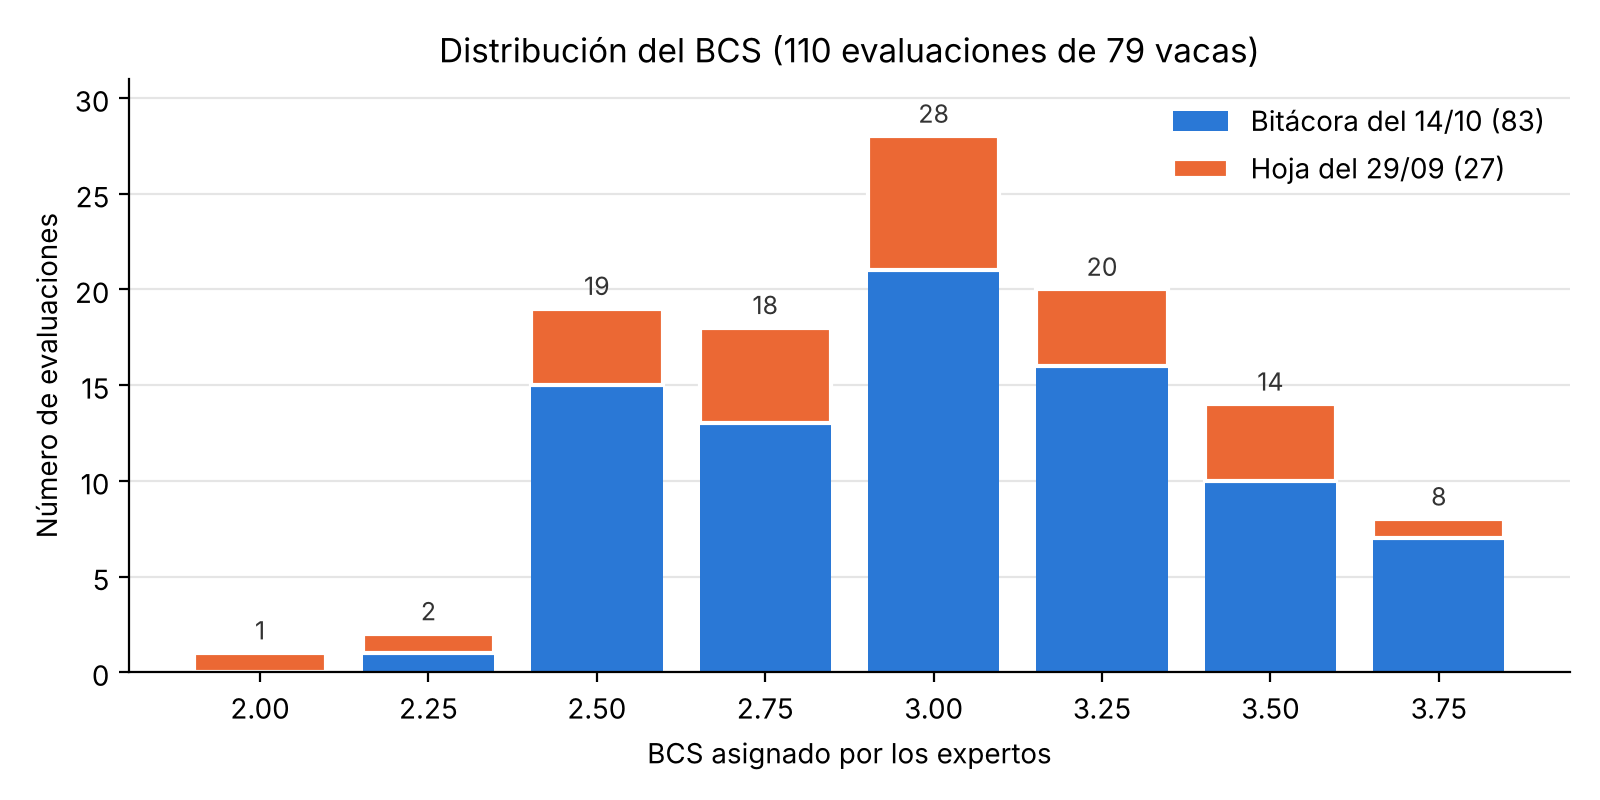
\includegraphics[width=0.85\textwidth]{figures/distribucion_bcs.png}
  \caption{Distribución del BCS asignado por los expertos.}
  \label{fig:distribucion-bcs}
\end{figure}

\begin{table}[H]
  \centering
  \caption{Evaluaciones por clase de BCS y fuente.}
  \label{tab:distribucion-bcs}
  \begin{tabular}{lrrrr}
    \toprule
    BCS & Bitácora 14/10 & Hoja 29/09 & Total & Porcentaje \\
    \midrule
    2.00 & 0 & 1 & 1 & 0.9\% \\
    2.25 & 1 & 1 & 2 & 1.8\% \\
    2.50 & 15 & 4 & 19 & 17.3\% \\
    2.75 & 13 & 5 & 18 & 16.4\% \\
    3.00 & 21 & 7 & 28 & 25.5\% \\
    3.25 & 16 & 4 & 20 & 18.2\% \\
    3.50 & 10 & 4 & 14 & 12.7\% \\
    3.75 & 7 & 1 & 8 & 7.3\% \\
    \midrule
    Total & 83 & 27 & 110 & 100\% \\
    \bottomrule
  \end{tabular}
\end{table}

La clase más frecuente es 3.0, con 28 evaluaciones (25.5\%). Las clases de los extremos tienen pocas evaluaciones, ya que 2.0 tiene 1, 2.25 tiene 2 y 3.75 tiene 8. No hay evaluaciones menores a 2.0 ni mayores a 3.75, así que el modelo no verá vacas fuera de ese rango.

Esta distribución es importante para las dos métricas que definimos. Con pocas vacas por clase, el porcentaje de predicciones dentro de $\pm0.25$ y $\pm0.50$ puede cambiar mucho con un solo error, y el MAE depende de qué tan lejos quedan las clases extremas del centro de la distribución.

\subsubsection*{Vacas con más de una evaluación}

En la bitácora del 14 de octubre hay 14 vacas con dos evaluaciones. La diferencia entre ellas es de 0.125 en promedio y de 0.25 como máximo, y en 7 vacas las dos evaluaciones son iguales. En la hoja hay 2 vacas con dos evaluaciones, la 1569 con una diferencia de 0.25 y la 1644 con evaluaciones iguales. Esto sirve como referencia de cuánto varía el BCS cuando lo asignan expertos distintos el mismo día.

Además, 15 vacas tienen BCS en las dos fechas. Entre el 29 de septiembre y el 14 de octubre su BCS difiere 0.225 en promedio (en valor absoluto) y 0.50 como máximo. En 5 vacas es igual y en 4 difiere más de 0.25, ya que la 1547 y la 1564 suben 0.5 del 29 de septiembre al 14 de octubre, la 1569 sube 0.375 y la 6137 baja 0.5. En conjunto no hay una tendencia, porque en promedio la hoja queda solo 0.008 por encima de la bitácora. Aun así, la diferencia máxima entre fechas (0.50) es el doble de la máxima entre expertos del mismo día (0.25), así que la fecha con la que se etiqueta cada foto importa.

\subsubsection*{Cruce entre fotos, conjunto de datos y BCS de expertos}

Cruzamos las 79 vacas con BCS con el conjunto de datos de VMS 3 (24 vacas) y con los datos de ordeño (34 vacas).

\begin{table}[H]
  \centering
  \caption{Cruce de las fuentes de datos.}
  \label{tab:cruce}
  \begin{tabular}{lr}
    \toprule
    Cruce & Vacas \\
    \midrule
    Con BCS de los expertos & 79 \\
    Con BCS y en VMS 3 & 20 \\
    Con BCS y con datos de ordeño & 12 \\
    En las tres fuentes & 2 (2082 y 8709) \\
    En VMS 3 sin BCS de los expertos & 4 (1570, 2165, 8769 y 91578) \\
    Con fotos y sin BCS & 2 (1549 y 1572) \\
    \bottomrule
  \end{tabular}
\end{table}

Las 20 vacas con BCS que están en VMS 3 son 1213, 1532, 1538, 1543, 1547, 1564, 1565, 1567, 1644, 2082, 2126, 2142, 6137, 6226, 8709, 8744, 8799, 91549, 91561 y 91576. Siete de ellas (1213, 1538, 1565, 1644, 2126, 6226 y 91576) solo tienen BCS de la hoja manuscrita.

De las 12 vacas con BCS de la bitácora que tienen valor en ``Evento BCS'', esta columna es mayor en 9, igual en 2 y menor en 1, y en promedio queda 0.43 puntos arriba. De las vacas que solo tienen BCS de la hoja, 4 tienen ``Evento BCS'', que es mayor en 3 e igual en 1. Como desconocemos qué mide esta columna, no se debe usar como si fuera el BCS de los expertos.

\subsubsection*{Relación con los datos de ordeño}

De las 34 vacas con datos de ordeño, 12 tienen BCS de los expertos, que son la 1204, 1221, 1554, 1624, 1634, 2076, 2082, 6178, 8709, 8729, 8758 y 8775. De ellas, solo la 2082 y la 8709 están también en VMS 3.

Los datos de ordeño siguen siendo contexto, porque cubren menos de la quinta parte de las vacas con BCS y sus fechas son de más de un año antes de las fotos. Por eso consideramos que su relación con el BCS no es significativa y no los usaremos como variables del modelo.

\subsubsection*{Exploración de los datos de ordeño (contexto)}

La tabla~\ref{tab:ordeno-resumen} resume las principales variables. La columna ``Global'' pondera a cada vaca por su número de ordeños. Las demás columnas comparan a las vacas entre sí y usan solo las 31 vacas con al menos 30 ordeños, porque tres vacas (1497, 8771 y 8775) tienen muy pocos datos para que sus promedios sean comparables.

\begin{table}[H]
  \centering
  \small
  \caption{Resumen de las variables de ordeño.}
  \label{tab:ordeno-resumen}
  \begin{tabularx}{\textwidth}{>{\raggedright\arraybackslash}Xrrrrr}
    \toprule
    Variable & Global & Media & Mediana & Mínimo & Máximo \\
    \midrule
    Ordeños por vaca & 7016 (34 vacas) & 206.4 & 244.5 & 1 & 419 \\
    Producción por ordeño (kg) & 13.72 & 13.53 & 13.86 & 7.66 & 18.85 \\
    Producción diaria (kg) & 31.12 & 30.45 & 28.13 & 13.15 & 55.50 \\
    Ordeños por día & 2.27 & 2.21 & 2.14 & 1.45 & 3.17 \\
    Duración media (min) & 8.48 & 8.24 & 7.83 & 5.36 & 13.51 \\
    Ordeños con patada (\%) & 18.5 & 18.2 & 15.2 & 0.7 & 62.2 \\
    Ordeños incompletos (\%) & 14.5 & 13.8 & 8.5 & 0.0 & 57.9 \\
    Ordeños con pezones no encontrados (\%) & 17.7 & 16.3 & 5.1 & 0.0 & 83.3 \\
    \bottomrule
  \end{tabularx}
\end{table}

La media, la mediana, el mínimo y el máximo son entre vacas. La producción diaria es la producción total entre los días en que la vaca tuvo al menos un ordeño.

\begin{figure}[H]
  \centering
  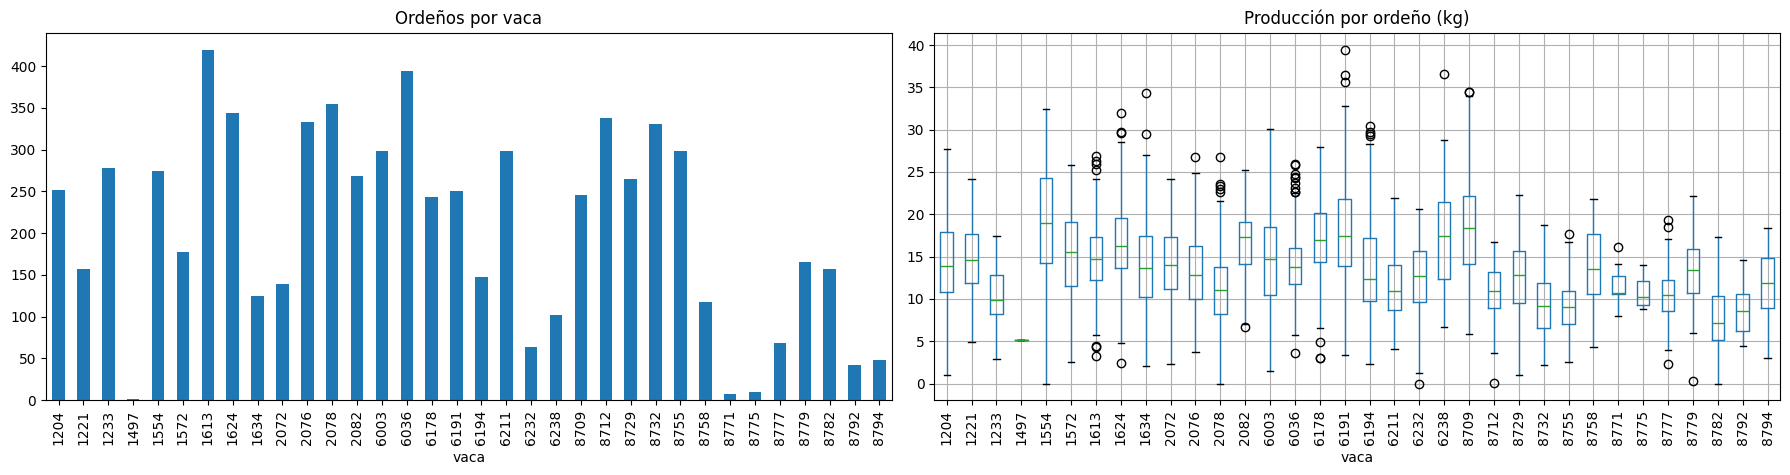
\includegraphics[width=\textwidth]{figures/ordenos_produccion_por_vaca.png}
  \caption{Ordeños por vaca y producción por ordeño (kg) de cada vaca.}
  \label{fig:ordenos}
\end{figure}

\begin{itemize}
  \item En producción, el promedio global fue de 13.7 kg por ordeño y la mediana entre vacas de 13.9 kg. La vaca con mayor promedio fue la 1554, con 18.9 kg por ordeño, y la de menor promedio entre las comparables fue la 8782, con 7.7 kg. Cinco vacas (1554, 2078, 6232, 8782 y 8712) tuvieron ordeños con 0 kg o 0.08 kg.
  \item En frecuencia y duración, las vacas se ordeñan en promedio 2.27 veces al día. El intervalo mediano entre ordeños va de 7.0 horas (vaca 6003) a 14.8 horas (vacas 8792 y 8794). Un ordeño dura en promedio 8.5 minutos. La vaca más rápida promedió 5.4 minutos (8712) y la más lenta 13.5 minutos (8755).
  \item Los incidentes se concentran en muy pocas vacas. Las vacas 8755, 8732 y 6003 tienen entre 45\% y 83\% de sus ordeños con pezones no encontrados o incompletos, y la 2076 tiene patada en el 62.2\% de sus ordeños.
  \item En la conductividad, la media por cuarto va de 3.82 mS/cm (TD) a 4.74 mS/cm (DD). Los ordeños con más de 6.0 mS/cm son pocos en todos los cuartos (entre 0.9\% y 2.8\%), pero se concentran en algunas vacas, como la 6178 en el cuarto DI (23.1\%).
  \item En cuanto a la sangre, solo 431 lecturas de cuarto tienen sangre mayor a 0 ppm, menos del 2\% del total.
  \item El estado AMD de la ubre vale 1 en 1050 de los 7016 ordeños (15.0\%). Por ahora solo consideramos su frecuencia, porque su significado debe confirmarse con el CAETEC.
  \item En cuanto a los robots, sobre las 7249 filas, VMS 3 registró 4276 (59.0\%), VMS 2 registró 1674 (23.1\%) y VMS 1 registró 1299 (17.9\%).
  \item En la cobertura temporal, 14 vacas tienen datos en prácticamente todo el rango de 140 días, 12 empiezan después del 01/03/2025 y 6 tienen ausencias prolongadas de entre 54 y 104 días. El socio formador explicó que esos huecos pueden corresponder al periodo seco de la vaca.
\end{itemize}

En cuanto al destino de la leche, la tabla~\ref{tab:destino} muestra a dónde fue la leche de los 7016 ordeños. Desviar la leche significa que su destino no es el tanque, donde se mezcla la leche de todas las vacas. Hubo 244 ordeños con leche desviada, de los cuales 152 fueron al drenaje y 92 a Divert 3. Según el socio formador, si la leche tiene sangre o microbios se desecha.

\begin{table}[H]
  \centering
  \caption{Destino de la leche.}
  \label{tab:destino}
  \begin{tabular}{lrr}
    \toprule
    Destino & Ordeños & Porcentaje \\
    \midrule
    Tanque & 6772 & 96.5\% \\
    Drenaje & 152 & 2.2\% \\
    Divert 3 & 92 & 1.3\% \\
    Total de ordeños & 7016 & 100\% \\
    \bottomrule
  \end{tabular}
\end{table}

Trece vacas enviaron menos del 95\% de su leche al tanque. El caso más destacable es la 6003, que solo envió el 71.5\% (213 de 298 ordeños). La columna ``Razón de la desviación'' tiene un único valor en todo el conjunto, así que no explica los 244 ordeños desviados.


\section{Verificar la calidad de los datos}

\subsection{Reporte de calidad de los datos}

\subsubsection*{Calidad de los datos de BCS}

\begin{itemize}
  \item De 761 archivos, 136 son copias dentro de la misma vaca, 122 en las carpetas del 14 de octubre y 14 en la carpeta de la vaca 91579 de la primera visita. En las carpetas del 14 de octubre, 13 vacas se descargaron dos veces con exactamente las mismas fotos y hay 18 archivos con nombre tipo ``IMG\_0530(1).HEIC''. En la primera visita hay 53 nombres con ``(1)'' y muchos de ellos son tomas distintas y no copias, por eso las copias se cuentan por huella y no por nombre. Ninguna foto del 29 de septiembre repite una foto del 14 de octubre.
  \item Las vacas 1548 y 2107 tienen 4 fotos iguales y no se sabe a cuál de las dos corresponde cada una. La 2107 no tiene más fotos.
  \item La vaca 2123 aparece dos veces en la bitácora con dos carpetas de fotos distintas, así que no se sabe qué fotos van con cada evaluación.
  \item Tres fotos de la carpeta de la vaca 1538 se llaman ``1538 y 8744\_atras'', por lo que no se sabe a cuál de las dos vacas corresponden.
  \item La carpeta de la vaca 1578 de la primera visita está vacía, aunque la vaca sí tiene fotos del 14 de octubre.
  \item De las 182 fotos JPG, 70 vienen con una orientación EXIF distinta de 1 y se verían giradas si el programa ignora esa etiqueta. Son 20 de las 24 fotos del Samsung S22 y 50 de las 117 fotos JPEG del iPhone 17 Pro Max de la primera visita.
  \item Hay dos formatos de imagen (HEIC y JPG) y 12 resoluciones distintas, y varias fotos de la primera visita son horizontales.
  \item La bitácora tiene 14 horas marcadas con ``x'' y 2 con otro formato, y la hoja no registra la hora. La hora no se usará en el modelo.
  \item Solo 20 de las 79 vacas con BCS están en el conjunto de datos de VMS 3.
  \item ``BCS ayer'' está vacía en las 24 vacas, mientras que ``Evento BCS'' tiene valores parecidos a un BCS. No sabemos si se relacionan ni qué significan.
  \item ``Evento BCS'' no coincide con el BCS de los expertos. De 12 vacas con ambos valores en la bitácora, el conjunto de datos es mayor en 9, igual en 2 y menor en 1. Las mayores diferencias son la vaca 8744 (3.0 contra 4.17), la 8799 (2.5 contra 3.5) y la 1547 (3.25 contra 3.98). No lo usaremos como etiqueta hasta aclarar qué mide y de qué fecha es.
  \item Dos vacas de la primera visita (1549 y 1572) tienen fotos pero no tienen BCS ni en la bitácora ni en la hoja.
  \item En la hoja, tres vacas tienen la nota ``Fresca'' pero VMS 3 las marca como preñada o inseminada, que son la 1565, la 8744 y la 91576.
  \item 15 vacas tienen BCS de las dos fechas y en 4 de ellas la diferencia es mayor a 0.25.
  \item Todas las filas de la bitácora tienen carpeta de fotos del 14 de octubre y todas esas carpetas tienen registro en la bitácora. De las vacas de la hoja, la 1578 y la 91561 no tienen fotos de la primera visita, aunque sí del 14 de octubre. No hay BCS vacíos, fuera del rango de 1 a 5 ni fuera de los pasos de 0.25 en ninguna de las dos fuentes.
\end{itemize}

\subsubsection*{Calidad de los datos de ordeño}

\begin{itemize}
  \item 233 filas tienen una acción distinta de ordeño (172 rechazadas y 61 echadas sin ordeñar). Se excluyen de las estadísticas de producción, incidentes y destino.
  \item 25 registros comparten vaca y hora de inicio con otro registro, así que pueden ser duplicados. De momento no se eliminan, por lo que los conteos pueden estar inflados hasta en 25 filas.
  \item Las columnas RCS y Usuario están vacías en las 34 vacas. No interpretamos el vacío de RCS como ausencia de mastitis, sino como que no se registró.
  \item La vaca 6211 (cuarto TI) y la 6232 (cuarto TD) no tienen lecturas en un cuarto. Según el socio formador, son cuartos que no se ordeñan por un problema de salud. Se mantienen como faltantes y no se imputan.
  \item Hay vacas con pocos datos, ya que la 1497 tuvo un ordeño, la 8771 tuvo 7 y la 8775 tuvo 10. Se excluyen de las comparaciones entre vacas.
  \item Hay ordeños con 0 kg en las vacas 1554, 2078, 6232 y 8782, y con 0.08 kg en la 8712. Falta revisar si son ordeños fallidos antes de modelar.
  \item Las columnas de patada, incompleto, pezones no encontrados y AMD de pezón están vacías entre el 82\% y el 89\% de las filas. No se tratan como faltantes, sino como ausencia del evento.
  \item En la conductividad, el rango común es de 3.0 a 5.0 mS/cm y usamos 6.0 mS/cm como valor alto.
\end{itemize}

\subsubsection*{Riesgos de las decisiones de etiqueta}

Evaluamos los riesgos con la misma escala del plan de riesgos de la fase 1. La probabilidad va de 0 a 100\%, el impacto de 1 a 5 y la magnitud es la probabilidad por el impacto. Con una magnitud de 1.5 o más mitigamos el riesgo, y con una menor lo aceptamos y lo monitoreamos.

\begin{table}[H]
  \centering
  \small
  \caption{Riesgos de las decisiones de etiqueta.}
  \label{tab:riesgos}
  \begin{tabularx}{\textwidth}{>{\raggedright\arraybackslash}p{0.33\textwidth}rrr>{\raggedright\arraybackslash}X}
    \toprule
    Riesgo & P & I & M & Decisión \\
    \midrule
    BCS distinto para la misma vaca (28 vacas con dos o más evaluaciones) & 90\% & 3 & 2.7 & Mitigar conservando las evaluaciones, entrenando con el promedio y evaluando contra cada una. \\
    \addlinespace
    Usar ``Evento BCS'' como etiqueta sin saber qué mide & 60\% & 5 & 3.0 & Mitigar usando solo el BCS de los expertos hasta que el socio confirme qué mide la columna. \\
    \addlinespace
    Nota ``Fresca'' contradictoria entre la hoja y el conjunto de datos & 75\% & 3 & 2.25 & Mitigar auditando con el CAETEC las 3 vacas en conflicto (1565, 8744 y 91576). \\
    \addlinespace
    Pocas vacas por clase de BCS, lo que vuelve inestables el MAE y los porcentajes dentro de $\pm0.25$ y $\pm0.50$ & 90\% & 4 & 3.6 & Mitigar separando entrenamiento y prueba por vaca y repartiendo las clases de BCS en los pliegues. \\
    \addlinespace
    Fotos duplicadas o asignadas a la vaca equivocada & 90\% & 4 & 3.6 & Mitigar detectando duplicados por contenido y excluyendo las fotos y vacas dudosas. \\
    \bottomrule
  \end{tabularx}
\end{table}

\subsection{Pendientes por aclarar}

\begin{itemize}
  \item Con Aurelio, qué mide ``Evento BCS'', por qué ``BCS ayer'' está vacía y de qué fecha es el archivo de VMS 3.
  \item Con Aurelio, qué significa el valor 6 de ``Número(s) de selección de animal''.
  \item Con Aurelio, qué es Divert 3 en los datos de ordeño y qué significa el valor 1 en el estado AMD.
  \item Con el CAETEC, el estado real de las vacas 1565, 8744 y 91576, que tienen la nota ``Fresca'' en la hoja y otro estado en VMS 3.
  \item Con quien subió las fotos de la primera visita, por qué la carpeta de la vaca 1578 está vacía y a qué vaca corresponden las fotos ``1538 y 8744\_atras''.
\end{itemize}

\subsubsection*{Diferencias entre cifras}

\begin{itemize}
  \item Hay 625 fotos asignadas a vacas y 621 fotos distintas. La diferencia son 4 fotos que están asignadas a las vacas 1548 y 2107. En este reporte usamos 625 al hablar de fotos por vaca y 621 al hablar de fotos únicas (peso, formato, cámara y resolución).
  \item Las 26 carpetas de la primera visita incluyen la carpeta vacía de la vaca 1578, por eso las fotos del 29 de septiembre vienen de 25 vacas.
  \item El peso de 2.18 GB incluye las copias y el de 1.80 GB cuenta cada foto única una sola vez.
\end{itemize}


\printbibliography

\end{document}
